\chapter{SYSTEM DESIGN}

\section{System Architecture Diagrams}

Figure~\ref{fig:testbed_arch} presents the complete one-page professional architecture of the testbed.

\begin{figure}[H]
\centering
\resizebox{\textwidth}{!}{%
\begin{tikzpicture}[
  node distance=1cm and 1.5cm,
  host/.style={draw, very thick, rounded corners=5pt, inner sep=12pt, fill=#1!5, draw=#1!50},
  vmpod/.style={draw, thick, rounded corners=2pt, fill=#1!20, draw=#1!80, font=\small\bfseries, align=center, inner sep=5pt},
  flow/.style={-{Stealth[length=3mm]}, thick, color=gray!80!black},
  lbl/.style={font=\scriptsize, fill=white, inner sep=1pt, color=gray!80!black}
]

  % KubeMaster Node
  \begin{scope}[local bounding box=master_box]
    \node[vmpod=corch] (agentic) {Agentic Orchestrator\\[0.1cm] \tiny (Observe $\to$ Think $\to$ Act)};
    \node[vmpod=cprom, right=1.2cm of agentic] (prom) {Prometheus \\\& Grafana};
    \node[vmpod=c5g, below=0.6cm of agentic] (llm) {LLM Backend\\(Ollama)};
    \draw[flow, <->] (agentic) -- node[lbl, left]{Inference} (llm);
    \draw[flow, <-] (agentic) -- node[lbl, above]{Metrics} (prom);
  \end{scope}
  \node[host=corch, fit=(master_box)(prom)(llm), label={[font=\bfseries, text=corch]north:KubeMaster Node (Control Plane)}] (master) {};

  % KubeWorker Node
  \begin{scope}[local bounding box=worker_box, shift={(0,-4.5)}]
    \node[vmpod=cembb] (upf1) {UPF-eMBB\\[0.1cm]\tiny (\texttt{tc} enforcement)};
    \node[vmpod=curllc, right=0.5cm of upf1] (upf2) {UPF-URLLC};
    \node[vmpod=cmmtc, right=0.5cm of upf2] (upf3) {UPF-mMTC};
    
    \node[vmpod=cembb, fill=cembb!8!white, below=0.6cm of upf1] (app1) {nginx App};
    \node[vmpod=curllc, fill=curllc!8!white, below=0.6cm of upf2] (app2) {NodeRED App};
    \node[vmpod=cmmtc,  fill=cmmtc!8!white, below=0.6cm of upf3] (app3) {Mosquitto App};

    \draw[flow] (upf1) -- (app1);
    \draw[flow] (upf2) -- (app2);
    \draw[flow] (upf3) -- (app3);
  \end{scope}
  \node[host=cembb, fit=(worker_box)(app3), label={[font=\bfseries, text=cembb]north:KubeWorker Node (Data Plane)}] (worker) {};

  % Open5GS Core VM
  \begin{scope}[local bounding box=core_box, shift={(9.5, 0)}]
    \node[vmpod=c5g, minimum width=2cm] (amf) {AMF};
    \node[vmpod=c5g, right=0.4cm of amf, minimum width=2cm] (nrf) {NRF / NSSF};
    \node[vmpod=c5g, below=0.6cm of amf, minimum width=2cm] (smf) {SMF (x3)};
    \node[vmpod=c5g, right=0.4cm of smf, minimum width=2cm] (udm) {UDM / AUSF};
  \end{scope}
  \node[host=c5g, fit=(core_box)(udm), label={[font=\bfseries, text=c5g]north:Open5GS Core VM}] (core) {};

  % UERANSIM VM
  \begin{scope}[local bounding box=ran_box, shift={(9.5, -4.5)}]
    \node[vmpod=cran, minimum width=3.5cm] (gnb) {gNB Emulator};
    \node[vmpod=cran, fill=cran!8!white, below=0.6cm of gnb, minimum width=3.5cm] (ue) {UEs (3 per slice)};
    \draw[flow, <->] (ue) -- node[lbl, left]{Uu Interface} (gnb);
  \end{scope}
  \node[host=cran, fit=(ran_box)(ue)(gnb), label={[font=\bfseries, text=cran]north:UERANSIM VM}] (ran) {};

  % Inter-host connections
  \draw[flow] (gnb.north) -- node[lbl, right]{N2 (NGAP)} (amf.south |- core.south);
  \draw[flow] (gnb.west) -- node[lbl, above]{N3 (GTP-U)} (upf3.east |- gnb.west);
  
  \draw[flow, dashed, color=corch, thick] (agentic.south) -- node[lbl, left, near end]{SSH QoS Config} (upf1.north);
  \draw[flow, dashed, color=cprom, thick] (worker.north -| prom.south) -- node[lbl, right]{Scrape} (prom.south);
  \draw[flow, dashed, color=c5g, thick] (smf.south) |- node[lbl, above, pos=0.8]{N4 (PFCP)} (upf2.north east);

\end{tikzpicture}}
\caption{Comprehensive Agentic Testbed Architecture, illustrating the physical separation of nodes and the decoupling of the multi-agent control loop from the 5G data plane.}
\label{fig:testbed_arch}
\end{figure}

Figure~\ref{fig:slice_arch} demonstrates the slicing architecture across the three isolated instances.

\begin{figure}[H]
\centering
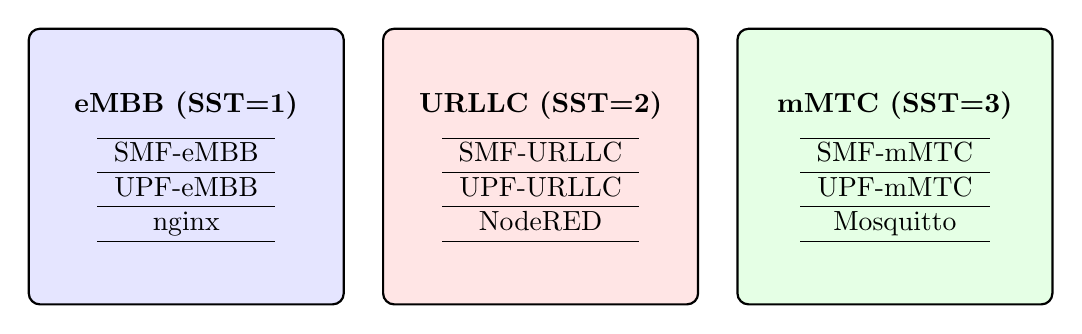
\begin{tikzpicture}[
  slice/.style={draw, rounded corners, thick, minimum width=4cm, minimum height=3.5cm, align=center}
]
\node[slice, fill=blue!10] (embb) at (0,0) {\textbf{eMBB (SST=1)}\\[0.2cm] \begin{tabular}{c} \hline SMF-eMBB \\ \hline UPF-eMBB \\ \hline nginx \\ \hline \end{tabular}};
\node[slice, fill=red!10] (urllc) at (4.5,0) {\textbf{URLLC (SST=2)}\\[0.2cm] \begin{tabular}{c} \hline SMF-URLLC \\ \hline UPF-URLLC \\ \hline NodeRED \\ \hline \end{tabular}};
\node[slice, fill=green!10] (mmtc) at (9,0) {\textbf{mMTC (SST=3)}\\[0.2cm] \begin{tabular}{c} \hline SMF-mMTC \\ \hline UPF-mMTC \\ \hline Mosquitto \\ \hline \end{tabular}};
\end{tikzpicture}
\caption{Slice Architecture showing complete isolation.}
\label{fig:slice_arch}
\end{figure}

Figure~\ref{fig:ue_flow} shows the UE Registration and Slice Selection sequence flow.

\begin{figure}[H]
\centering
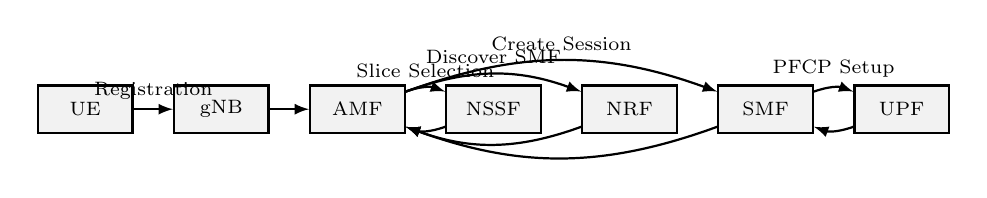
\begin{tikzpicture}[
  agent/.style={draw, thick, minimum width=1.2cm, minimum height=0.6cm, fill=gray!10, font=\scriptsize},
  msg/.style={-latex, thick}
]
\matrix[column sep=0.5cm, row sep=0.8cm] {
\node[agent] (ue) {UE}; & \node[agent] (gnb) {gNB}; & \node[agent] (amf) {AMF}; & \node[agent] (nssf) {NSSF}; & \node[agent] (nrf) {NRF}; & \node[agent] (smf) {SMF}; & \node[agent] (upf) {UPF}; \\
};
\draw[msg] (ue) -- node[above, font=\scriptsize] {Registration} (gnb);
\draw[msg] (gnb) -- (amf);
\draw[msg] (amf) edge[bend left=20] node[above, font=\scriptsize] {Slice Selection} (nssf);
\draw[msg] (nssf) edge[bend left=20] (amf);
\draw[msg] (amf) edge[bend left=20] node[above, font=\scriptsize] {Discover SMF} (nrf);
\draw[msg] (nrf) edge[bend left=20] (amf);
\draw[msg] (amf) edge[bend left=20] node[above, font=\scriptsize] {Create Session} (smf);
\draw[msg] (smf) edge[bend left=20] node[above, font=\scriptsize] {PFCP Setup} (upf);
\draw[msg] (upf) edge[bend left=20] (smf);
\draw[msg] (smf) edge[bend left=20] (amf);
\end{tikzpicture}
\caption{UE Registration \& Slice Selection Flow.}
\label{fig:ue_flow}
\end{figure}

\section{MEC Architecture}

Figure~\ref{fig:mec_locality} proves MEC traffic locality (local breakout).

\begin{figure}[H]
\centering
\begin{tikzpicture}[
  box/.style={draw, rounded corners, thick, minimum width=3cm, minimum height=1cm, align=center, fill=gray!10},
  arrow/.style={-latex, thick, line width=1.5pt}
]
\node[box] (ue) {UE};
\node[box, below=1cm of ue] (upf) {UPF};
\node[box, below=1cm of upf] (app) {Application};
\node[right=2cm of upf, font=\bfseries, color=red] (wan) {NO INTERNET / WAN};
\draw[arrow] (ue) -- (upf);
\draw[arrow] (upf) -- (app);
\draw[arrow, red, dashed] (upf) -- (wan);
\end{tikzpicture}
\caption{MEC Traffic Locality with local breakout.}
\label{fig:mec_locality}
\end{figure}

Figure~\ref{fig:k8s_deploy} illustrates the Kubernetes deployment diagram.

\begin{figure}[H]
\centering
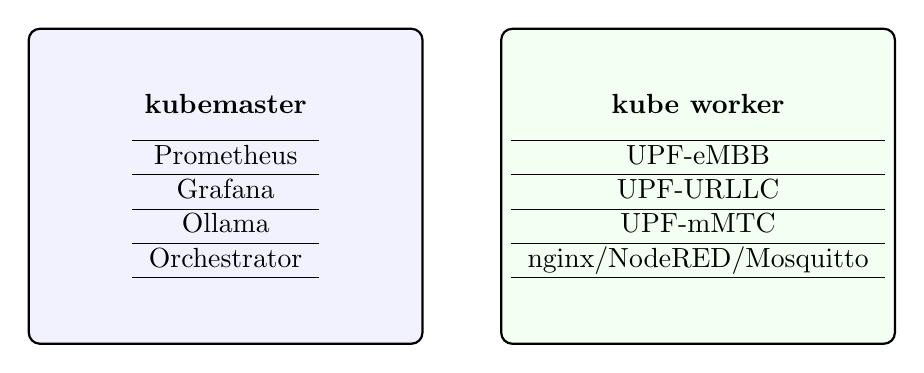
\begin{tikzpicture}[
  nodebox/.style={draw, rounded corners, thick, minimum width=5cm, minimum height=4cm, align=center}
]
\node[nodebox, fill=blue!5] (master) at (0,0) {\textbf{kubemaster}\\[0.3cm] \begin{tabular}{c} \hline Prometheus \\ \hline Grafana \\ \hline Ollama \\ \hline Orchestrator \\ \hline \end{tabular}};
\node[nodebox, fill=green!5] (worker) at (6,0) {\textbf{kube worker}\\[0.3cm] \begin{tabular}{c} \hline UPF-eMBB \\ \hline UPF-URLLC \\ \hline UPF-mMTC \\ \hline nginx/NodeRED/Mosquitto \\ \hline \end{tabular}};
\end{tikzpicture}
\caption{Kubernetes Deployment Diagram.}
\label{fig:k8s_deploy}
\end{figure}

\section{Control Loop}

Figure~\ref{fig:closed_loop} illustrates the Closed Loop QoS Control mechanism.

\begin{figure}[H]
\centering
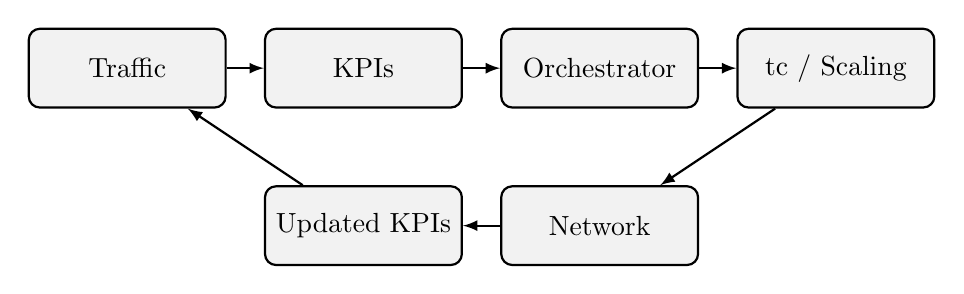
\begin{tikzpicture}[
  box/.style={draw, rounded corners, thick, minimum width=2.5cm, minimum height=1cm, align=center, fill=gray!10},
  arrow/.style={-latex, thick}
]
\node[box] (traffic) at (0,0) {Traffic};
\node[box] (kpis) at (3,0) {KPIs};
\node[box] (orch) at (6,0) {Orchestrator};
\node[box] (tc) at (9,0) {tc / Scaling};
\node[box] (net) at (6,-2) {Network};
\node[box] (ukpis) at (3,-2) {Updated KPIs};

\draw[arrow] (traffic) -- (kpis);
\draw[arrow] (kpis) -- (orch);
\draw[arrow] (orch) -- (tc);
\draw[arrow] (tc) -- (net);
\draw[arrow] (net) -- (ukpis);
\draw[arrow] (ukpis) -- (traffic);
\end{tikzpicture}
\caption{Closed Loop QoS Control.}
\label{fig:closed_loop}
\end{figure}

Figure~\ref{fig:tc_enf} identifies the \texttt{tc} enforcement point at the UPF.

\begin{figure}[H]
\centering
\begin{tikzpicture}[
  box/.style={draw, rounded corners, thick, minimum width=3cm, minimum height=1cm, align=center, fill=orange!10},
  arrow/.style={-latex, thick}
]
\node[box] (ue) {UE};
\node[box, below=0.8cm of ue] (gtp) {GTP-U};
\node[box, below=0.8cm of gtp] (upf) {UPF};
\node[box, below=0.8cm of upf, fill=red!10] (tun) {ogstun-embb\\(TBF)};
\node[box, below=0.8cm of tun] (app) {App};

\draw[arrow] (ue) -- (gtp);
\draw[arrow] (gtp) -- (upf);
\draw[arrow] (upf) -- (tun);
\draw[arrow] (tun) -- (app);
\end{tikzpicture}
\caption{\texttt{tc} Enforcement Point.}
\label{fig:tc_enf}
\end{figure}
\section{Six Research Contributions}
\begin{contribbox}{Project Contributions}
\begin{enumerate}[noitemsep,leftmargin=*]
  \item \textbf{C1 — Autonomous QoS Orchestration Framework}: A cloud-native, closed-loop system that enforces per-slice QoS on live 5G traffic without human intervention.
  \item \textbf{C2 — LangGraph Multi-Agent Architecture}: A stateful five-node agent graph (Observe$\to$Think$\to$Validate$\to$Act$\to$Reflect) coordinating specialised agents.
  \item \textbf{C3 — Chain-of-Thought Network Reasoning}: A mandatory JSON CoT schema requiring \texttt{root\_cause\_assessment} and \texttt{lever\_validity} before any control action.
  \item \textbf{C4 — Wrong-Lever Avoidance Mechanism}: A rolling relative-load metric ($\rho_{\text{eMBB}}$) that prevents erroneous eMBB throttling when eMBB is idle.
  \item \textbf{C5 — Memory-Assisted Decision Making}: A persistent ring-buffer Agent Memory injecting empirical action-outcome history into every LLM prompt.
  \item \textbf{C6 — Comparative Evaluation}: A pre-registered three-scenario behavioral audit comparing Agentic vs.\ Rule-Based controllers on live testbed traffic.
\end{enumerate}
\end{contribbox}

%% ─────────────────────────────────────────────────────────────
\section{Seven-Layer System Architecture}

Figure~\ref{fig:sevenlayer} presents the complete end-to-end architecture across seven logical layers.

\begin{figure}[H]
\centering
\resizebox{\textwidth}{!}{%
\begin{tikzpicture}[
  lyr/.style={draw, rounded corners=5pt, very thick,
              minimum width=22cm, minimum height=1.55cm,
              fill=#1!7, draw=#1!55},
  pod/.style={draw, rounded corners=3pt, fill=#1!22, draw=#1!65,
              font=\scriptsize\bfseries, minimum width=2.4cm,
              minimum height=0.65cm, align=center},
  ifc/.style={font=\tiny\ttfamily, text=gray},
  arr/.style={-{Stealth[length=3mm]}, thick, #1},
  lbl/.style={font=\bfseries\scriptsize, rotate=90, text=#1}
]
%% ── Layer backgrounds (bottom=L1, top=L7)
\foreach \i/\col/\name in {
  0/cmmtc/{Layer 1: 5G User Plane},
  1/cran/{Layer 2: Radio Access Network},
  2/c5g/{Layer 3: 5G Core Network},
  3/cembb/{Layer 4: Kubernetes Data Plane},
  4/cqos/{Layer 5: QoS Enforcement},
  5/cprom/{Layer 6: Observability Stack},
  6/corch/{Layer 7: Agentic Orchestration}
}{
  \node[lyr=\col] (L\i) at (11, \i*1.75+0.87) {};
  \node[\col, font=\bfseries\scriptsize, left=0.1cm of L\i.west, rotate=90] {\name};
}

%% ── L1: User Plane
\node[pod=cmmtc] at (5,  0.87) {eMBB UEs (3)\\HLS Video};
\node[pod=curllc] at (11, 0.87) {URLLC UEs (3)\\HTTP Telemetry};
\node[pod=cmmtc]  at (17, 0.87) {mMTC UEs (3)\\MQTT Publish};

%% ── L2: RAN
\node[pod=cran] at (5,  2.62) {UERANSIM gNB};
\node[pod=cran] at (9,  2.62) {uesimtun0--8\\(TUN Interfaces)};
\node[pod=cran] at (13.5, 2.62) {NR-UE Emulation\\(9 sessions)};
\node[ifc] at (11, 1.5) {Uu (NR air interface / TUN)};

%% ── L3: 5G Core
\node[pod=c5g] at (3,  4.37) {AMF\\(NGAP)};
\node[pod=c5g] at (7,  4.37) {SMF-eMBB\\SMF-URLLC\\SMF-mMTC};
\node[pod=c5g] at (12, 4.37) {NRF / NSSF};
\node[pod=c5g] at (17, 4.37) {UDM / AUSF};
\node[ifc] at (11, 3.2) {N1/N2 (NGAP/NAS) \quad N4 (PFCP)};

%% ── L4: K8s Data Plane
\node[pod=cembb]  at (4,   6.12) {UPF-eMBB\\(10.45.0.0/16)};
\node[pod=curllc] at (9,   6.12) {UPF-URLLC\\(10.46.0.0/16)};
\node[pod=cmmtc]  at (14,  6.12) {UPF-mMTC\\(10.47.0.0/16)};
\node[pod=c5g]    at (19,  6.12) {Kubernetes\\Worker Node};
\node[ifc] at (11, 4.95) {N3 (GTP-U) \quad PFCP Session};

%% ── L5: QoS Enforcement
\node[pod=cqos] at (4,   7.87) {HTB Root\\rate 1000mbit};
\node[pod=cembb] at (8.5,7.87) {Class 1:10 eMBB\\rate=\textbf{var}};
\node[pod=curllc] at (13,7.87) {Class 1:20 URLLC\\prio=1};
\node[pod=cmmtc] at (17.5,7.87){Class 1:30 mMTC\\rate=10mbit};
\node[ifc] at (11, 6.75) {TUN egress → tc HTB qdisc};

%% ── L6: Observability
\node[pod=cprom] at (5,  9.62) {Prometheus\\:9090};
\node[pod=cgraf]  at (11, 9.62) {Grafana\\:3000};
\node[pod=cprom]  at (17, 9.62) {tun-metrics\\DaemonSet};
\node[ifc] at (11, 8.6) {metrics scrape (:9100, :9200)};

%% ── L7: Orchestration
\node[pod=corch] at (2.5,11.37) {Monitoring\\Agent};
\node[pod=corch] at (6.5, 11.37) {Planning\\Agent (LLM)};
\node[pod=corch] at (10.5,11.37) {Validation\\Gate};
\node[pod=corch] at (14.5,11.37) {Execution\\Agent};
\node[pod=corch] at (18.5,11.37) {Agent\\Memory};
\node[ifc] at (11, 10.35) {State Vector → CoT → Validated Action → tc command};

%% ── Vertical interface arrows (between layer centers)
\draw[arr=cran]  (11,1.75) -- (11,2.2);
\draw[arr=c5g]   (11,3.5)  -- (11,3.95);
\draw[arr=cembb] (11,5.25) -- (11,5.7);
\draw[arr=cqos]  (11,7.0)  -- (11,7.45);
\draw[arr=cprom] (11,8.75) -- (11,9.2);
\draw[arr=corch] (11,10.5) -- (11,10.95);

%% ── Feedback: Orchestrator → QoS (SSH tc command)
\draw[arr=corch, bend right=15, dashed, thick]
  (14.5,11.0) to node[right, ifc, pos=0.5]{SSH tc change} (4,8.2);

%% ── Observability → Orchestrator
\draw[arr=cprom, bend left=10, dashed]
  (5,10.0) to node[left, ifc, pos=0.5]{Prometheus metrics} (2.5,11.0);

\end{tikzpicture}}
\caption{Seven-Layer End-to-End System Architecture. Solid arrows denote data-plane flows; dashed arrows denote control and observability flows.}
\label{fig:sevenlayer}
\end{figure}

%% ─────────────────────────────────────────────────────────────
\section{Agentic Orchestration Framework}

\begin{figure}[H]
\centering
\resizebox{\textwidth}{!}{%
\begin{tikzpicture}[
  agent/.style={draw, rounded corners=6pt, fill=#1!10, draw=#1!65,
                very thick, minimum width=3.6cm, minimum height=1.5cm,
                align=center, font=\small\bfseries},
  sub/.style={draw, rounded corners=3pt, fill=#1!18, draw=#1!50,
              font=\scriptsize\ttfamily, minimum width=3.2cm,
              minimum height=0.55cm, align=center},
  arr/.style={-{Stealth[length=3.5mm]}, thick, #1},
  lbl/.style={font=\scriptsize, fill=white, inner sep=2pt, align=center}
]

%% Agents
\node[agent=cprom]  (mon)  at (0,0)    {Monitoring Agent\\(Observe)};
\node[agent=corch]  (plan) at (6,0)    {Planning Agent\\(Think)};
\node[agent=cqos]   (val)  at (12,0)   {Validation Gate\\(Validate)};
\node[agent=curllc] (exec) at (12,-4)  {Execution Agent\\(Act)};
\node[agent=cgraf]  (mem)  at (6,-4)   {Agent Memory\\(Reflect)};

%% Sub-labels
\node[sub=cprom, below=0.1cm of mon]  {RTT / TP / PDR\\embb\_load\_fraction};
\node[sub=corch, below=0.1cm of plan] {CoT JSON:\\root\_cause + lever};
\node[sub=cqos,  below=0.1cm of val]  {bounds + contradiction\\confidence adj.};
\node[sub=curllc,below=0.1cm of exec] {\texttt{tc class change}\\via SSH};
\node[sub=cgraf, below=0.1cm of mem]  {(State, Action, $\Delta$RTT)\\ring-buffer depth=10};

%% Main pipeline
\draw[arr=c5g]   (mon)  -- node[lbl, above]{State Vector}   (plan);
\draw[arr=corch] (plan) -- node[lbl, above]{CoT Plan}        (val);
\draw[arr=cqos]  (val)  -- node[lbl, right]{Valid Action}    (exec);
\draw[arr=cgraf] (exec) -- node[lbl, above]{Action + Result} (mem);

%% Memory ↔ Planner feedback
\draw[arr=cgraf, dashed, bend left=20]
  (mem.north) to node[lbl, right]{Context Injection} (plan.south);

%% Monitor ← memory update
\draw[arr=cprom, dashed, bend right=25]
  (mem.west) to node[lbl, below, pos=0.4]{Next Cycle} (mon.south);

\end{tikzpicture}}
\caption{LangGraph Multi-Agent Orchestration Pipeline (Contribution C2). Each node is a specialised agent; dashed arrows represent cross-cycle feedback.}
\label{fig:langgraph_pipeline}
\end{figure}

%% ─────────────────────────────────────────────────────────────
\section{Individual Agent Architecture}

\subsection{Monitoring Agent}
\begin{figure}[H]
\centering
\begin{tikzpicture}[
  src/.style={draw, rounded corners=3pt, fill=#1!15, draw=#1!60,
              font=\scriptsize, minimum width=2.8cm, minimum height=0.6cm, align=center},
  box/.style={draw, rounded corners=4pt, fill=gray!10, draw=gray!50,
              font=\scriptsize\bfseries, minimum width=3.2cm, minimum height=0.7cm, align=center},
  arr/.style={-{Stealth[length=2.5mm]}, thick, gray!70}
]
\node[src=cprom] (prom)  at (0,4)   {Prometheus\\scrape :9090};
\node[src=cran]  (ssh)   at (4,4)   {SSH log parser\\UERANSIM RTT};
\node[src=cembb] (proc)  at (8,4)   {\texttt{/proc/net/dev}\\GTP-U counters};

\node[box] (agg) at (4,2.5) {Metric Aggregator\\(threading.Lock)};
\node[box] (frac) at (4,1)  {Load Fraction: $\rho_{\text{eMBB}}(t) = \tfrac{\lambda(t)}{\max_{W}\lambda}$};
\node[box] (cache) at (4,-0.3) {State Cache (3-second update)};

\draw[arr] (prom)  -- (agg);
\draw[arr] (ssh)   -- (agg);
\draw[arr] (proc)  -- (agg);
\draw[arr] (agg)   -- (frac);
\draw[arr] (frac)  -- (cache);
\node[font=\scriptsize, right=0.5cm of cache, text=corch]
  {$\rightarrow$ Planning Agent};
\end{tikzpicture}
\caption{Monitoring Agent Architecture (Contribution C4). Three input collectors feed an aggregator; the derived load-fraction metric is written to the thread-safe state cache.}
\label{fig:mon_agent}
\end{figure}

\subsection{Planning Agent}
\begin{figure}[H]
\centering
\begin{tikzpicture}[
  box/.style={draw, rounded corners=4pt, fill=#1!12, draw=#1!55,
              font=\scriptsize\bfseries, minimum width=3.0cm, minimum height=0.65cm, align=center},
  arr/.style={-{Stealth[length=2.5mm]}, thick, gray!70},
  lbl/.style={font=\scriptsize, text=gray}
]
\node[box=cprom] (state) at (0,3.5)   {Current State Vector};
\node[box=cgraf]  (mem)  at (5,3.5)   {Memory Context\\(last 10 decisions)};
\node[box=corch] (prompt) at (2.5,2.2) {Structured Prompt\\(sys + state + memory)};
\node[box=corch] (llm)   at (2.5,0.9) {LLM Inference\\(llama3.2:3b)};
\node[box=cqos]  (cot)   at (2.5,-0.4){CoT JSON Output:\\root\_cause, lever\_validity,\\action, rate, confidence};

\draw[arr] (state) -- (prompt);
\draw[arr] (mem)   -- (prompt);
\draw[arr] (prompt) -- (llm);
\draw[arr] (llm)   -- (cot);
\end{tikzpicture}
\caption{Planning Agent Architecture (Contributions C3, C5). State and memory are injected into a structured prompt; the LLM generates a mandatory CoT schema.}
\label{fig:plan_agent}
\end{figure}

\subsection{Validation Gate}
\begin{figure}[H]
\centering
\begin{tikzpicture}[
  box/.style={draw, rounded corners=4pt, fill=#1!12, draw=#1!55,
              font=\scriptsize\bfseries, minimum width=3.2cm, minimum height=0.65cm, align=center},
  arr/.style={-{Stealth[length=2.5mm]}, thick, gray!70},
  lbl/.style={font=\scriptsize, text=gray}
]
\node[box=corch] (in)   at (0,0)    {CoT JSON from\\Planning Agent};
\node[box=cqos]  (rng)  at (4,1.2)  {Range Clamp:\\50–1000 Mbit};
\node[box=curllc](cdet) at (4,0)    {Contradiction\\Detector};
\node[box=cqos]  (conf) at (4,-1.2) {Confidence\\Adjustment};
\node[box=cmmtc] (out)  at (8,0)    {Approved Action\\+ adjusted confidence};

\draw[arr] (in)  -- (rng);
\draw[arr] (in)  -- (cdet);
\draw[arr] (in)  -- (conf);
\draw[arr] (rng)  -- (out);
\draw[arr] (cdet) -- node[lbl,above]{\textit{if contradiction}: $c \gets 0.5c$} (conf);
\draw[arr] (conf) -- (out);
\end{tikzpicture}
\caption{Validation Gate Architecture (Contribution C4). Contradiction detection catches logical inconsistencies between the \texttt{root\_cause\_assessment} and the proposed action.}
\label{fig:val_gate}
\end{figure}

%% ─────────────────────────────────────────────────────────────
\section{Mathematical Foundations}

Table~\ref{tab:notation} defines the notation used throughout this report.

\begin{table}[H]
\centering
\caption{Mathematical Notation}
\label{tab:notation}
\begin{tabularx}{\textwidth}{llX}
\toprule
\textbf{Symbol} & \textbf{Unit} & \textbf{Definition} \\
\midrule
$\rho_{\text{eMBB}}(t)$ & — & eMBB relative load fraction at time $t$ \\
$\lambda(t)$  & pkt/s  & eMBB packet rate at time $t$ \\
$W$           & cycles & Rolling window size (default: 8) \\
$R(t)$        & ms     & URLLC RTT$_{99}$ at time $t$ \\
$\theta$      & ms     & URLLC SLA threshold (20\,ms) \\
$r(t)$        & Mbit/s & eMBB \texttt{tc} rate cap at time $t$ \\
$r_{\max}$    & Mbit/s & Maximum eMBB rate (1000\,Mbit) \\
$T_{\text{rec}}$ & s   & SLA recovery time \\
$C_{\text{sla}}$ & —   & SLA compliance ratio \\
$\eta_{\text{act}}$ & — & Action efficiency \\
$N_T$         & —      & Total monitoring cycles \\
$N_V$         & —      & Cycles with SLA violation ($R > \theta$) \\
\bottomrule
\end{tabularx}
\end{table}

\subsection{eMBB Load Fraction}

The eMBB relative load fraction is the central metric enabling Contribution C4. Unlike absolute throughput, it is invariant to traffic profile differences:

\begin{equation}
\rho_{\text{eMBB}}(t) = \frac{\lambda(t)}{\displaystyle\max_{t' \in [t-W\Delta, t]} \lambda(t')}
\label{eq:load_frac}
\end{equation}

where $\Delta = 3$\,s is the monitoring interval and $W = 8$ is the rolling window. $\rho_{\text{eMBB}} \in [0, 1]$; a value $< 0.2$ indicates a low-activity slice that should not be throttled regardless of RTT.

\subsection{SLA Compliance Ratio}

\begin{equation}
C_{\text{sla}} = 1 - \frac{N_V}{N_T} = \frac{\#\{t : R(t) \leq \theta\}}{N_T}
\label{eq:sla_comp}
\end{equation}

\subsection{Recovery Time}

Recovery time is the interval from the first SLA breach until the RTT falls back below $\theta$:

\begin{equation}
T_{\text{rec}} = t_{\text{clear}} - t_{\text{breach}}, \quad t_{\text{clear}} = \min\{t > t_{\text{breach}} : R(t) \leq \theta\}
\label{eq:trec}
\end{equation}

\subsection{Throughput Preservation Ratio}

\begin{equation}
\text{TP} = 1 - \frac{\displaystyle\sum_{t: r(t) < r_{\max}} (r_{\max} - r(t)) \cdot \Delta}{\displaystyle r_{\max} \cdot N_T \cdot \Delta}
\label{eq:tp}
\end{equation}

\subsection{Action Efficiency}

The fraction of throttle actions that followed a genuine SLA violation or rising trend:

\begin{equation}
\eta_{\text{act}} = \frac{\#\{\text{throttle}: R > \theta \text{ or trend rising}\}}{\#\{\text{throttle actions}\}}
\label{eq:eff}
\end{equation}

%% ─────────────────────────────────────────────────────────────
\section{Control Loop State Transition Diagram}

\begin{figure}[H]
\centering
\begin{tikzpicture}[
  state/.style={draw, circle, minimum size=2.6cm, font=\small\bfseries,
                align=center, thick, fill=#1!15, draw=#1!60},
  arr/.style={-{Stealth[length=3mm]}, thick},
  lbl/.style={font=\scriptsize, align=center, fill=white, inner sep=2pt}
]
\node[state=cmmtc]  (N)  at (0,0)    {NORMAL\\$r=r_{\max}$};
\node[state=cqos]   (P)  at (5,2)    {PRE-\\CONG.};
\node[state=curllc] (C)  at (10,0)   {CONGESTED\\$R>\theta$};
\node[state=cprom]  (T)  at (10,-4)  {THROTTLED\\$r<r_{\max}$};
\node[state=cembb]  (R)  at (5,-4)   {RECOVERING};

\draw[arr,cqos]  (N) -- node[lbl,above left]{$\rho\uparrow$, trend rising} (P);
\draw[arr,curllc](P) -- node[lbl,above right]{$R>\theta$} (C);
\draw[arr,cprom, bend right=20] (P.east) to node[lbl,right,pos=0.4]{pre-emptive\\throttle (C4)} (T.north);
\draw[arr,curllc](C) -- node[lbl,right]{throttle} (T);
\draw[arr,cembb] (T) -- node[lbl,below]{stable (C5\\memory cue)} (R);
\draw[arr,cmmtc] (R) -- node[lbl,below left]{$r=r_{\max}$} (N);
\draw[arr,curllc,bend right=20,dashed](C.north west) to node[lbl,above,pos=0.55]{WLA: $\rho<0.2$\\no throttle (C4)} (N.north east);
\draw[arr,curllc,bend left=15](R.east) to node[lbl,right]{breach} (T.west);
\end{tikzpicture}
\caption{Orchestrator Control Loop State Machine. WLA = Wrong-Lever Avoidance (C4). The dashed path is structurally impossible in rule-based systems.}
\label{fig:fsm}
\end{figure}
